\documentclass[letterpaper,10pt]{article}
\usepackage[T1]{fontenc}
\usepackage[utf8]{inputenc}
\usepackage{lmodern}
\usepackage{amsmath}
\usepackage{cancel}
\usepackage[margin=1.1in]{geometry}
\usepackage{verbatim}
\usepackage{scrextend}
\usepackage{longtable}
\usepackage{framed}
\usepackage{amssymb}
\usepackage{wasysym}
\usepackage{multicol}
\usepackage{graphicx}
\usepackage{color}
\usepackage{caption}
\usepackage{subcaption}
\usepackage{float}
\usepackage{fancyhdr}
\usepackage[utf8]{inputenc}
\usepackage[mathletters]{ucs}
\usepackage{hyperref}
\usepackage{tikz,tkz-euclide}
\usepackage{pstricks,pst-plot,pst-node,pstricks-add}

\hypersetup
{
  colorlinks=false,
	pdfborder={0 0 0}
}


\pagestyle{fancy}
\lhead{Joseph Mate - jmate - 20246021}
\rhead{CS 648 - Professor Ilyas - UI Optimizer}
\DeclareRobustCommand\iff{\;\Longleftrightarrow\;}

\begin{document}

\raggedright

\setlength{\columnseprule}{0.5pt}


\section{Introduction}
The Postgres query planner does not necessarily return a good plan even with
interesting orders. As mentioned in the CORDS paper, one reason is the estimated
number of rows returned by a scan or join can be way off \cite{Ilyas04} due to
the independence assumption falling apart. \\[0.5cm]

For instance, if there are many clauses that are dependant on each other,
the optimizer might estimate one row because of the independence assumption of
AND clauses. As a result, the optimizer might perform a nested loop join because
the single row fits in memory. An example where clause could be looking for rows
belonging to a particular city in a province in a country on a continent. None
of the values are independent and as a result their individual probabilities
should not be multiplied.  \\[0.5cm]

As a result, this prototype was created to explore the possibility of a database
user manually manipulating the plan, or changing the estimates of the number of
rows returned from a base or joined relation. The primary use case is for
queries that are expected to take hours or days to complete. Additionally, this
tool can be used for queries that are expected to be used many times. If used in
other settings, then the time spent having the user optimize the query may
significantly exceed the time saved in query processing.

\section{Features}
The prototype begins by displaying the plan that the optimizer initially
computes. The UI can display any number of levels of joins. From that UI, you
can change which join algorithm should be applied on the two relations. Lastly,
the UI also allows you to modify the estimated number of rows for each relation
and then the query planner searches for a new plan using the new estimates.

\section{How it Works}
The most complicated components of this project are summarized here. A lot of
other challenges encountered are not included here to keep the report brief.

\subsection{UI}
The UI was built using GTK+. The most complicated component of the UI is the
display of the plan. This was solved by applying a table GUI abstraction, where
a plan node widget can be placed at any row and column of the table. A tree
structure can be simulated in the table. The following diagram illustrates how
the formula was derived.

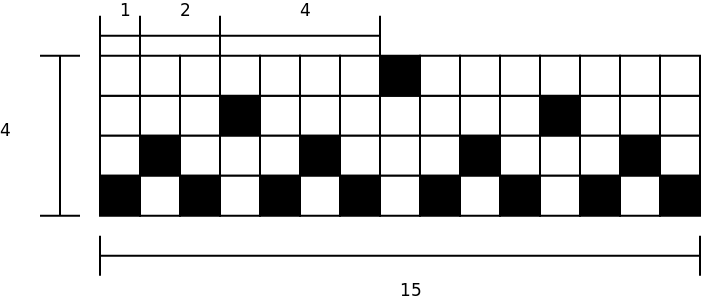
\includegraphics[scale=0.5]{table-derivation.png}

The 0th row is the top most row of the table. The 0th column is the left most
column of the table. Given the above convention, we can compute the position of
all the nodes using the following recursive formulae \\
\begin{align*}
	row_{root} & = 0 \\
	column_{root} & = 2^{TreeHeight-1}-1 \\
	row_{child} & = row_{parent} + 1 & \mbox { for both left and right children}\\
	column_{child} & = column_{parent} - 2^{height_{parent}-2} & \mbox { for the left child} \\
	column_{child} & = column_{parent} + 2^{height_{parent}-2} & \mbox { for the right child} \\
\end{align*}

This can generalize to n-ary trees if needed. First, determine the max number of
branches, then rederive the above formulas with n instead of two.

\subsection{Changing Joins}
The prototype wraps the plan tree data structure returned by query planner inside
its own tree so that each node of the tree has pointers to any important GUI
widgets that the user may have manipulated. When the user changes the join on
the GUI, we recursively rebuild the path upwards starting from the node that was
changed. This updates the costs all the way up. The user can select one of the
joins populated in the drop down list and hit the change button to replace the
join with the one selected. A screenshot
is provided below.

\begin{center}
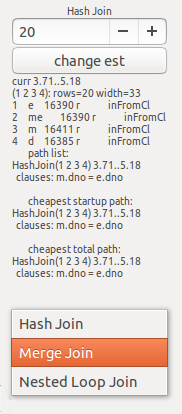
\includegraphics[scale=0.7]{join-ddl.png}
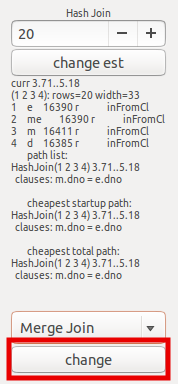
\includegraphics[scale=0.7]{join-ddl-selected.png}
\end{center}

\subsection{Changing a Relation's Rows Estimates}
The prototype adds a hashtable to the PlannerInfo struct. The hashtable is a map
from relids belonging to the relation accumulated so far in the tree to the
overridden estimated number of rows. If the hashtable does not contain an entry
for the given relids, then the estimate for that relation has not been overridden.
Where ever the estimated number of rows was accessed in costsize.c, a lookup to
the hashtable to check if it has been overridden prepended. Additionally, the
following functions also check for overridden estimates:
\textit{set\_baserel\_size\_estimates, set\_joinrel\_size\_estimates, and
get\_parameterized\_joinrel\_size}. Lastly, the user changes the estimated number of
rows by changing the textbox provided inside the GUI widget representing that
relation and then hits . A screenshot below is provided for reference.

\begin{center}
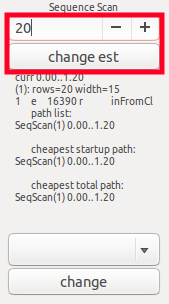
\includegraphics[scale=0.7]{change-estimate.png}
\end{center}


\section{Future Work}
Firstly, in order to focus on the functionality of this prototype, the GUI runs
on the database process, This avoided having to implement a communication
protocol between the database and client and figuring out how to serialize that
data. Secondly, there is no way to manipulate the structure of the tree.
Thirdly, the user cannot change which scan should be performed on a base
relation. Fourthly, only one path-key is considered for the merge join. A
variety of options should be presented to the user selecting merge join. Lastly,
there is absolutely no validation to assist the user when he creates something
that does not make sense.

\section{Acknowledgements}
I would like to thank José Calvo for recommending that I place the GUI directly
on the database server so that I would not have to figure out how to serialize
data between the server and client.

\nocite{*}               
\bibliographystyle{plain}
\bibliography{write-up}     


\end{document}
